\documentclass[tikz,border=4pt]{standalone}
% Paleta y fuentes compartidas por el libro y las figuras (única fuente de verdad).
\RequirePackage{xcolor}
\definecolor{oxido}{HTML}{B7410E}
\definecolor{cobre}{HTML}{D27D2D}
\definecolor{carbon}{HTML}{2B2B2B}
\definecolor{azul}{HTML}{1F5F8B}
\definecolor{arena}{HTML}{F4EDE4}

\usepackage{fontspec}
\setsansfont{FiraSans}[Extension=.otf,UprightFont=*-Regular,BoldFont=*-SemiBold,ItalicFont=*-Italic,BoldItalicFont=*-SemiBoldItalic]
\setmonofont{FiraMono}[Extension=.otf,UprightFont=*-Regular,BoldFont=*-Medium,Scale=0.95]
\usetikzlibrary{positioning,arrows.meta,calc,fit}
\begin{document}
\sffamily\small
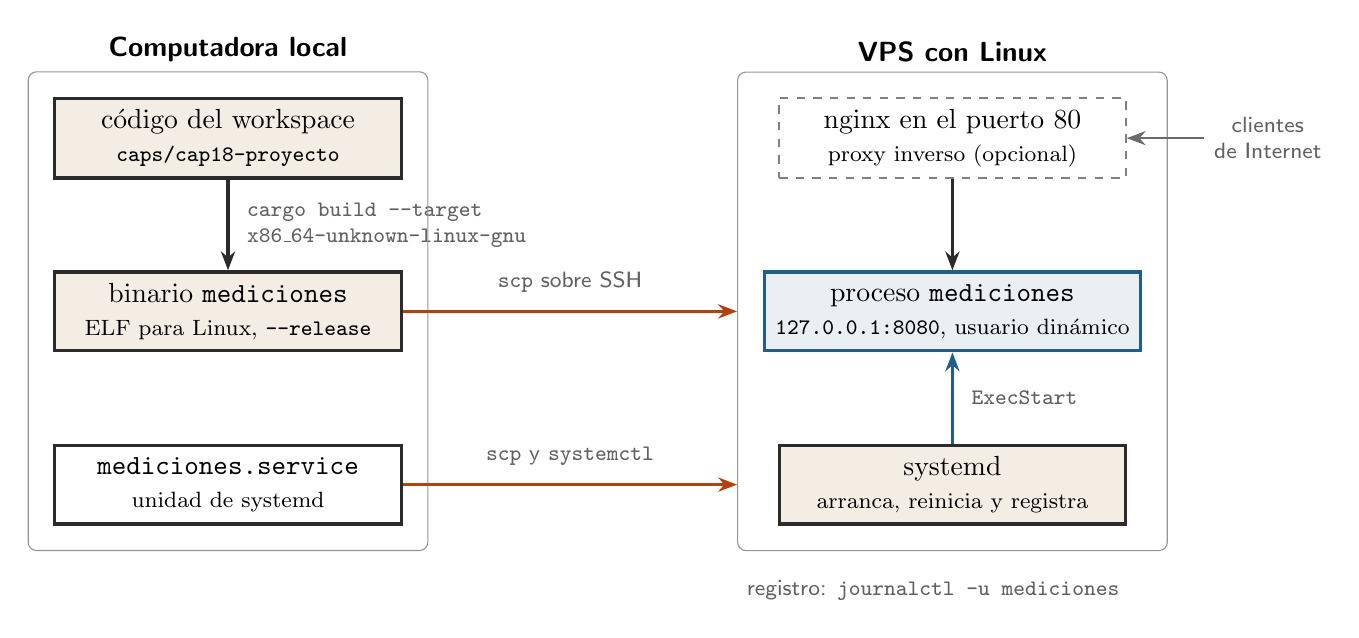
\begin{tikzpicture}[>={Stealth[length=2.4mm]},
  execute at begin node={\hyphenpenalty=10000},
  caja/.style={draw=carbon,very thick,fill=arena,align=center,
    minimum width=44mm,minimum height=10mm,inner sep=4pt},
  proc/.style={draw=azul,very thick,fill=azul!10,align=center,
    minimum width=44mm,minimum height=10mm,inner sep=4pt},
  opc/.style={draw=carbon!60,thick,dashed,fill=white,align=center,
    minimum width=44mm,minimum height=10mm,inner sep=4pt},
  rotulo/.style={font=\sffamily\footnotesize,text=carbon!75},
  titulo/.style={font=\sffamily\bfseries}]
  % Máquina local
  \node[caja] (src) at (0,0) {código del workspace\\\footnotesize\texttt{caps/cap18-proyecto}};
  \node[caja] (bin) at (0,-2.2) {binario \texttt{mediciones}\\\footnotesize ELF para Linux, \texttt{-{}-release}};
  \draw[->,very thick,carbon] (src) -- node[rotulo,right=3pt,align=left]
    {\texttt{cargo build -{}-target}\\\texttt{x86\_64-unknown-linux-gnu}} (bin);
  \node[caja,fill=white] (svc) at (0,-4.4) {\texttt{mediciones.service}\\\footnotesize unidad de systemd};
  \node[draw=carbon!50,rounded corners=3pt,inner sep=9pt,fit=(src)(bin)(svc)(svc.south)] (local) {};
  \node[titulo,anchor=south] at (local.north) {Computadora local};
  % VPS
  \node[opc] (nginx) at (9.2,0) {nginx en el puerto 80\\\footnotesize proxy inverso (opcional)};
  \node[proc] (proc) at (9.2,-2.2) {proceso \texttt{mediciones}\\\footnotesize\texttt{127.0.0.1:8080}, usuario dinámico};
  \node[caja] (sysd) at (9.2,-4.4) {systemd\\\footnotesize arranca, reinicia y registra};
  \node[draw=carbon!50,rounded corners=3pt,inner sep=9pt,fit=(nginx)(proc)(sysd)] (vps) {};
  \node[titulo,anchor=south] at (vps.north) {VPS con Linux};
  \draw[->,very thick,carbon] (nginx) -- (proc);
  \draw[->,very thick,azul] (sysd) -- node[rotulo,right=3pt] {\texttt{ExecStart}} (proc);
  % Copia
  \draw[->,very thick,oxido] (bin.east) -- node[rotulo,above=3pt] {\texttt{scp} sobre SSH}
    (bin.east -| vps.west);
  \draw[->,very thick,oxido] (svc.east) -- node[rotulo,above=3pt] {\texttt{scp} y \texttt{systemctl}}
    (svc.east -| vps.west);
  % Internet
  \node[rotulo,align=center,anchor=west] (net) at (12.4,0) {clientes\\de Internet};
  \draw[->,thick,carbon!70] (net.west) -- (nginx.east);
  \node[rotulo,align=left,anchor=north west] at ($(vps.south west)+(0,-0.25)$)
    {registro: \texttt{journalctl -u mediciones}};
\end{tikzpicture}
\end{document}
